\chapter{Foundations}
\label{chap:2}

This chapter presents the theory applied in this thesis. First, the details of the communication problem are described briefly to put the theory into perspective, and then the mathematical background of the frameworks used to model this problem is introduced. 

\section{Problem Formulation}
\label{sec:prob_formulation}

\begin{wrapfigure}{r}{5cm}
	\begin{center}
		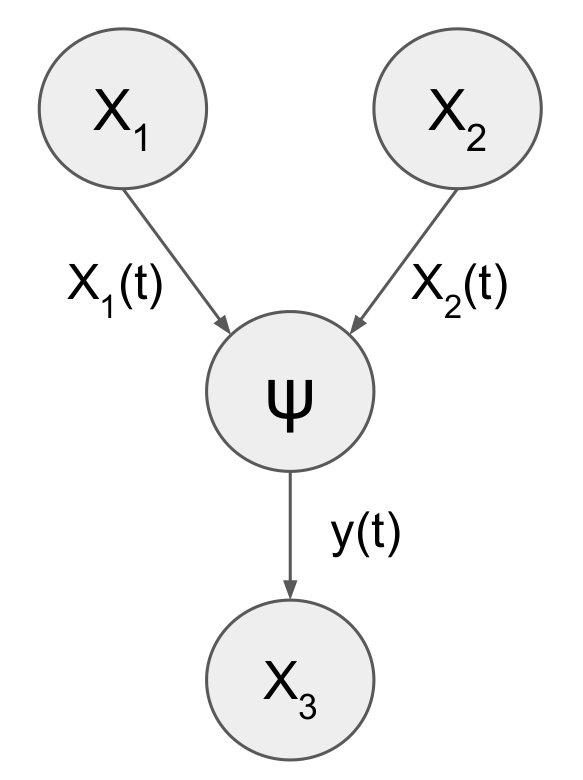
\includegraphics[width=3.5cm]{figures/simple_graph}
		\caption{Communication model.}
		\label{fig:graph_model}
	\end{center}
\end{wrapfigure} 
The communication model considered in this work is given in \cref{fig:graph_model}. The parent nodes, $X_{1}$ and $ X_{2}$, emit messages which contain information about their states. These messages are translated by an observation model, $\psi$, and an agent node, $ X_{3} $ makes a decision based on this translated message, $ y $. The main objective is to infer the observation model, given a set of trajectories of nodes.\\
The transition models of the nodes and the dependencies between them are modelled as a continuous-time Bayesian network (CTBN), denoted by S. \\%The network S represents a stochastic process over a structured multivariate state space $ \rchi = [\rchi_1,..., \rchi_n] $. \\
The messages that are emitted by the parent nodes $X_{1}$ and $ X_{2} $ are modelled as independent homogeneous continuous-time Markov processes $X_{i}(t)$, with state space $ \rchi_{i} = \left\lbrace x_{1}, x_{2}, ..., x_{m} \right\rbrace  $ for $ i \in \left\lbrace 1,2 \right\rbrace $.\\
The agent node $ X_3 $ does not have direct access to the messages but observes a translation of them. The observation model is defined as the likelihood of a translation given the parent messages.
\begin{equation}
\psi(x_1, x_2) \coloneqq p(y(t) \mid X_{1}(t)=x_1, X_{2}(t)=x_2)
\end{equation}
The agent  $ X_{3} $ is modelled as inhomogeneous continuous-time Markov process with state space $ \rchi_{3} = \left\lbrace x_{1}, x_{2}, ..., x_{m} \right\rbrace  $ and set of actions $ a \in \left\lbrace a_{0}, a_{1}, ..., a_{k}\right\rbrace  $ to choose from. \\
Given the observation, the agent forms a belief over the parent states, $  b(x_{1}, x_{2}; t) $, that summarizes the past observations. The policy of the agent, $ \pi(a \mid b) $, is assumed to be shaped by evolution (close) to optimality. Based on the belief state, the agent takes an action, which in the setting described above corresponds to changing its internal dynamics. 

\section{Continuous-Time Bayesian Networks}
\label{sec:ctbn_intro}
Consider a directed acyclic graph denoted by $ \mathcal{G} = \left( \mathcal{V}, \mathcal{E}\right) $, where $ \mathcal{V} $ is a set of nodes and $ \mathcal{E} \subseteq \mathcal{V} \times \mathcal{V} $ is a set of edges such that $ \mathcal{E} = \left\lbrace \left( m, n\right) : m, n \in \mathcal{V} \right\rbrace $. In this graph, the parent nodes of node n are defined as the set of nodes that feed into it and denoted by $ \mathrm{Par}_{\mathcal{G}}(n) = \left\lbrace m \in \mathcal{V} : \left( m, n \right) \in \mathcal{E} \right\rbrace $. A directed acyclic graph is characterized as a Bayesian network where each node respresents a random variable such that $ \mathcal{V} = \left\lbrace X_1, X_2, ...., X_N\right\rbrace  $ and the joint distribution $ p(X_1, X_2, ..., X_N) $ factors as 
\begin{equation}
p(X_1, X_2, ..., X_N) = \prod_{i=1}^{N} p(X_i \mid \mathrm{Par}_{\mathcal{G}}(X_i)).
\end{equation}
A continuous-time Bayesian network (CTBN) is a graphical model with graph $\mathcal{G} = \left( \mathcal{V}, \mathcal{E}\right) $ that represents a collection of random variables whose values evolve continuously over time. In the CTBN framework, the dependencies of a set of Markov processes (MPs) can be modelled efficiently through a directed graph, relying on two assumptions. The first assumption is that only one node can transition at a time, and the second is that the instantaneous dynamics of each node depends only on its parent nodes \cite{Cohn2010a, Nodelman1995}. A two component CTBN is illustrated in \autoref{fig:ctbn_visuals}.
\begin{figure}[H] 
	\centering
	\resizebox{.8\textwidth}{!}{
		\begin{subfigure}{.33\textwidth}
			\centering
			\resizebox{.25\textwidth}{!}{
				\begin{tikzpicture}
				\tikzstyle{var} = [draw, circle, minimum size=.5cm]
				\tikzstyle{arrow} = [-latex, line width=0.5pt]
				
				\node [var] (x1) {$X_1$};
				\node [var, below=0.7cm of x1] (x2) {$X_2$};
				\node [below=0.1cm of x2] (t) {};
				
				\draw [arrow] (x1) to (x2);
				\end{tikzpicture}
			}
			\caption{}
		\end{subfigure}
		\begin{subfigure}{.66\textwidth}
			\centering
			\resizebox{.90\textwidth}{!}{
				\begin{tikzpicture}
				\tikzstyle{var} = [draw, circle, minimum size=.5cm]
				\tikzstyle{arrow} = [-latex, line width=0.5pt]
				
				\node [var] (x1) {};
				\node [left=0.3cm of x1] (x1_l) {$ X_1 $};
				\node [var, right=1cm of x1] (x1_h) {};
				\node [var, right=1cm of x1_h] (x1_2h) {};
				\node [var, right=1cm of x1_2h] (x1_3h) {};
				\node [right=1cm of x1_3h] (x1_4h) {...};
				
				\node [var, below=1cm of x1] (x2) {};
				\node [left=0.3cm of x2] (x2_l) {$ X_2 $};
				\node [below=0.1cm of x2] (t) {$ t $};
				\node [var, right=1cm of x2] (x2_h) {};
				\node [below=0.1cm of x2_h] (t+h) {$ t+h $};
				\node [var, right=1cm of x2_h] (x2_2h) {};
				\node [below=0.1cm of x2_2h] (t+2h) {$ t+2h $};
				\node [var, right=1cm of x2_2h] (x2_3h) {};
				\node [below=0.1cm of x2_3h] (t+3h) {$ t+3h $};
				\node [right=1cm of x2_3h] (x2_4h) {...};
				
				\draw [arrow] (x1) to (x2_h);
				\draw [arrow] (x1_h) to (x2_2h);
				\draw [arrow] (x1_2h) to (x2_3h);
				\draw [arrow] (x1_3h) to (x2_4h);
				
				\draw [arrow] (x1) to (x1_h);
				\draw [arrow] (x1_h) to (x1_2h);
				\draw [arrow] (x1_2h) to (x1_3h);
				\draw [arrow] (x1_3h) to (x1_4h);
				
				\draw [arrow] (x2) to (x2_h);
				\draw [arrow] (x2_h) to (x2_2h);
				\draw [arrow] (x2_2h) to (x2_3h);
				\draw [arrow] (x2_3h) to (x2_4h);
				
				\end{tikzpicture}
			}
			\caption{}
		\end{subfigure}
	}
	\caption[Two component CTBN]{Two component CTBN. (a) Network representation (b) CTBN in (a) unrolled in time as $ h\rightarrow 0 $}
	\label{fig:ctbn_visuals}
\end{figure}

\subsection{Continuous-Time Markov Processes}
A continuous-time Markov process (CTMP) is a continuous-time stochastic process which satisfies the Markov property, namely, the probability distribution over the states at a later time is conditionally independent of the past states given the current state \cite{Cohn2010a}. \\
Consider a CTMP X(t) over a single variable with a countable state space $ \rchi $. Then the Markov property can be written as
\begin{equation}
\operatorname{Pr}\left(X(t_{k})=x_{t_{k}} \mid X(t_{k-1})=x_{t_{k-1}}, \ldots, X(t_{0})=x_{t_{0}}\right)=\operatorname{Pr}\left(X(t_{k})=x_{t_{k}} \mid X(t_{k-1})=x_{t_{k-1}}\right)
\end{equation}
where X(t) denotes the state of the variable at time $ t $ such that $ X(t)=x_t \in \rchi, t \geq 0$, and $ t_0<t_1<...<t_k $.\\
A CTMP is represented by its transition intensity matrix, $ \textbf{Q} : \rchi \times \rchi \rightarrow \mathbb{R}$. In this matrix, the intensity $ q_{i} $ represents the instantaneous probability of leaving state $ x_{i} $ and $ q_{i,j} $ represents the instantaneous probability of switching from state $ x_{i} $ to $ x_{j} $, where $ x_i, x_j \in \rchi $. 
\begin{equation}
\textbf{Q} = 
\begin{bmatrix}
-q_{1} & q_{1,2} &     {\hdots}  & q_{1,n} \\
q_{2,1} & -q_{2} &     {\hdots}  & q_{2,n}  \\
{\vdots}  &     {\vdots}  &     {\ddots}  & {\hdots}  \\
q_{n,1} &  q_{n,2} &  {\hdots} & -q_{n}
\end{bmatrix}
\label{eq:Q_matrix}
\end{equation}
where $ q_{i} = \sum_{i \neq j} q_{i,j}$ \cite{Nodelman1995}.

\subsubsection{Homogenous Continuous-Time Markov Processes}
A continuous-time Markov process is time-homogenous when the transition intensities do not depend on time. Let X(t) be a homogenous CTMP, with a countable state space $ \rchi $ and transition intensity matrix $ \textbf{Q} $. Infinitesimal transition probability from state $ x_{i} $ to $ x_{j} $ in terms of the transition intensities $ q_{i,j} $ can be written as \cite{Cohn2010a}:
\begin{equation}
p_{i,j}(h)=\delta_{ij}+q_{i,j} h+o(h)
\label{eq:Markov_trans_func}
\end{equation}
where $ p_{i, j}(h) \equiv \operatorname{Pr}(X(t+h)=x_j\mid X(t)=x_i) $ are Markov transition functions, $ \delta_{i,j} = \delta(x_i,x_j)$ is Kronecker delta and $ o(\cdot) $ is a function decaying to zero faster than its argument such that $ \lim_{h \to 0} \frac{o(h)}{h} = 0 $.\\
The \textit{Chapman-Kolmogorov-} or \textit{master-equation} is then derived as follows:
\begin{align}
p_{j}(t) &= \operatorname{Pr}(X(t) = x_{j}) \nonumber\\
& =\sum_{\forall i} p_{i, j}(h) p_{i}(t-h) \nonumber \\
\lim_{h\rightarrow 0} p_{j}(t) 
& = \lim_{h\rightarrow 0} \sum_{\forall i} \left[ \delta_{ij}+q_{i,j} h+o(h)\right]  p_{i}(t-h) \nonumber \\ 
& = \lim_{h\rightarrow 0} p_{j}(t-h) + \lim_{h\rightarrow 0} h \sum_{\forall i} q_{i,j} p_{i}(t-h) \nonumber \\
\lim_{h\rightarrow 0} \frac{p_{j}(t) - p_{j}(t-h)}{h} 
&= \lim_{h\rightarrow 0} \sum_{\forall i} q_{i,j} p_{i}(t-h) \nonumber\\
\frac{d}{dt} p_{j}(t) & = \sum_{\forall i} q_{i,j} p_{i}(t)
%        & = \sum_{\forall i \neq j}\left[  q_{i,j} p_{i}(t) - q_{j,i} p_{j}(t) \right]\nonumber
\label{eq:master_equation}
\end{align}
Equation \ref{eq:master_equation} can be written in matrix form:
\begin{equation}
\frac{d}{dt} p(t) = p(t)\textbf{Q}
\end{equation}
where the time-dependent probability distribution $ p(t) $ is a row vector with entries $ \left\lbrace p_{i}(t)\right\rbrace_{x_{i}\in \rchi} $. The solution of the system of ordinary differential equations (ODEs) is
\begin{equation}
p(t)=p(0) \exp (t\textbf{Q})
\label{eq:ode_sol}
\end{equation}
with initial distribution $ p(0) $.\\
The amount of time staying in a state $ x_{i} $ is exponentially distributed with parameter $ q_{i} $. The probability density function $ f $ and cumulative distribution function $ F $ for staying in the state $ x_{i} $ can be written as \cite{Nodelman1995}
\begin{align}
f(t) & = q_{i} \exp \left(-q_{i} t\right), t\geq 0  \label{eq:f(t)_homo}\\
F(t) & = 1 - \exp \left(-q_{i} t\right), t\geq 0 .
\end{align}
Given the transitioning from state $ x_{i} $, the probability of landing on state $ x_{j} $ is $ q_{i,j}/q_{i} $.
\paragraph*{Likelihood Function}
\label{sec:llh_of_homo}
Consider a single transition denoted as $ d = <x_{i},x_{j},t> $, where the transition occurs from state $ x_{i} $ to $ x_{j} $ after spending t amount of time at state $ x_{i} $. The likelihood of this transition is the product of the probability of having remained at state $ x_{i} $ for duration $ t $ from \autoref{eq:f(t)_homo}, and the probability of transitioning to $ x_{j} $.
\begin{equation}
p(d  \mid \textbf{Q}) = \left( q_{i}\exp(-q_{i}t) \right) \left( \frac{q_{i,j}}{q_{i}} \right)
\end{equation}
The likelihood of a trajectory sampled from a homogenous CTMC, denoted by $ X^{[0,T]} $, can be decomposed as the product of the likelihood of single transitions. The sufficient statistics summarizing this trajectory can be written as $ T[x_{i}] $, the total amount of time spent in state $ x_{i} $ and  $ M[x_{i}, x_{j}] $ the total number of transitions from state $ x_{i} $ to $ x_{j} $. 
\begin{align}
M[x_i,x_j] & = \sum_{d \in X^{[0,T]}} \mathbb{1}(X(t)=x_i)\mathbb{1}(X(t+h)=x_j)\\
T[x_i] &= \sum_{d \in X^{[0,T]}} \mathbb{1}(X(t)=x_i)
\end{align}
where $ \mathbb{1}(\cdot) $ is the indicator function. Then the likelihood of a trajectory $  X^{\left[0,T\right] } $ can be written as:
\begin{align}
p(X^{[0,T]}  \mid \textbf{Q}) &=  \prod_{d \in X^{[0,T]}} p(d \mid \textbf{Q}) \nonumber\\&=\left(\prod_{ i} q_{i}^{M[x_{i}]} \exp \left(-q_{i} T[x_{i}]\right)\right)\left(\prod_{ i} \prod_{ j \neq i} \left(\frac{q_{i,j}}{q_{i}}\right)^{M\left[x_{i}, x_{j}\right]}\right) \nonumber\\ & = \prod_{j \neq i}  \exp(-q_{i,j}T[x_{i}])\ q_{i,j}^{M[x_{i},x_{j}]}
\label{eq:lh_traj_homo}
\end{align}
where $ M[x_{i}] = \sum_{j \neq i} M[x_{i}, x_{j}] $ is the total number transitions leaving state $ x_{i} $.

\subsubsection{Conditional Markov Processes}
A continuous-time Markov process is \textit{time-inhomogenous} when the transition intensities change over time. In a CTBN, while every node is a Markov process, the leaf nodes are characterized as \textit{conditional} Markov processes, a type of inhomogeneous MP, where the intensities change over time, but not as a function of time rather as a function of parent states \cite{Nodelman1995}. \\
Let X be a conditional Markov process in a graph $ \mathcal{G} $, with a set of parents $ U = \mathrm{Par}_{\mathcal{G}}(X)$. Its \textit{conditional intensity matrix} (CIM) $ \textbf{Q}_{X\given U} $ can be viewed as a set of homogenous intensity matrices $ \textbf{Q}_{X\given u} $, with entries $ q_{i,j \mid u} $ (similar to \autoref{eq:Q_matrix}), for each instantiation of parent nodes $ U(t) =u $ such that $ u \in \mathcal{U} = ⨉_{X_m \in \mathrm{Par}_{\mathcal{G}(X)}} \rchi_m $, where $ ⨉ $ denotes Cartesian product \cite{Nodelman1995}. As a result, given a trajectory of parent nodes, X has a trajectory of intensity matrix as
\begin{equation}
\textbf{Q}^{[0,T]} = [\textbf{Q}_{X\given U(t_0)}, \textbf{Q}_{X\given U(t_1)}, ..., \textbf{Q}_{X\given U(t_N)}],\ 0<t_0<...<t_N\leq T\text{.}
\end{equation}
Markov transition function for a conditional MP can be written as
\begin{align}
\operatorname{Pr}(X(t + h) = x_j \mid X(t)=x_i, U(t)=u, \textbf{Q}_{X\given u}) = \delta(i,j) + q_{i,j \mid u} h + o(h).
\label{eq:CIM_trans_funct}
\end{align}

\paragraph*{Likelihood Function}
Given the instantiation of its parents, the complete information on the dynamics of X is obtained. Then the likelihood of a trajectory drawn from a conditional MP $ X $ can be written similar to \autoref{eq:lh_traj_homo},
\begin{align}
p(X^{[0,T]}  \mid \textbf{Q}_{X\given U}) &=  \left(\prod_{ u}\prod_{ i} q_{i\mid u}^{M[x_{i}\mid u]} \exp \left(-q_{i\mid u} T[x_{i}\mid u]\right)\right)\left(\prod_{ u}\prod_{ i} \prod_{ j \neq i} \left(\frac{q_{i,j\mid u}}{q_{i\mid u}}\right)^{M\left[x_{i}, x_{j}\mid u\right]}\right) \nonumber\\ & = \prod_{ u}\prod_{j\neq i}  \exp(-q_{i,j\mid u}T[x_{i}\mid u]) \ q_{i,j\mid u}^{M[x_{i},x_{j}\mid u]}
\label{eq:lh_traj_cond}
\end{align}
with the sufficient statistics, $ T[\cdot] $ and $ M[\cdot] $ introduced in \cref{sec:llh_of_homo}, are also conditioned on parent nodes.

\subsection{The CTBN Model}
Evidently, a homogeneous CTMP can be considered as a conditional MP whose set of parents is empty. Thus, a CTBN can be formed as a set of conditional Markov processes.\\
Let S be a CTBN with graph $ \mathcal{G} = (\mathcal{V}, \mathcal{E}) $ and local variables $ \mathcal{V} = \left\lbrace X_1, X_2, ..., X_N\right\rbrace  $, each with a state space $ \rchi_n $. This results in factorizing state spaces for S such that $ \mathcal{S} = 
\rchi_1 \times \rchi_2\times ...\times \rchi_N $. The joint states of the variables are denoted by $ s = (x_1, x_2, ..., x_N) \in \mathcal{S}$ where $ x_1 \in \rchi_1, ..., x_N \in \rchi_N $. The dependencies of each variable are defined as a set of its parents $ U_n = \mathrm{Par}_{\mathcal{G}}(X_n) $ with values $ U_n(t) = u_n $ such that $ u_n \in \mathcal{U}_n = ⨉_{X_m \in \mathrm{Par}_{\mathcal{G}(X_n)}} \rchi_m $. In the following, the set of all conditional transition intensity matrices are denoted as $ \textbf{\textit{Q}} = \left\lbrace Q_{X_1 \given U_1}, ..., Q_{X_N \given U_N}\right\rbrace  $.\\
Consider a trajectory drawn from S, such that $ S^{[0, T]} = \left\lbrace X_1^{[0,T]},  X_2^{[0,T]}, ...,  X_N^{[0,T]}\right\rbrace  $. Following \autoref{eq:lh_traj_cond}, the likelihood of this trajectory can be written as
\begin{align}
p( S  \mid \textbf{\textit{Q}} ) = \prod_{n=1}^{N} \prod_{u \in \mathcal{U}_{n}} \prod_{x_i \in \mathcal{X}_{n}} \prod_{x_j \in \mathcal{X}_{n} \backslash x_i}
\exp \left(q_{i,j\mid u}^{n} T_{n}[x_i\mid u]\right) (q_{i,j\mid u}^{n})^{M_{n}[x_i, x_j\mid u]}
\label{eq:lh_CTBN}
\end{align}
where $ T_n[\cdot] $ and $ M_n[\cdot] $ indicates the sufficient statistics for $ X_n $. \\
It should be noted that a CTBN can also be represented by a single conditional intensity matrix, through \textit{amalgamation} operation \cite{Nodelman1995}.
\section{Partially Observable Markov Decision Processes}
\label{sec:belief_POMDP}
The partially observable Markov decision process (POMDP) framework provides a model of an agent which interacts with its environment but is unable to obtain certain information about its state. Instead, the agent gets an observation which is a function of the true state, e.g. noisy observations, translation. The main goal, similar to Markov decision processes (MDPs), is to learn a policy solving a task by optimizing a reward function. \\
The problem of decision making under uncertainty can be considered in two parts for the agent. The first is to keep a belief state which summarizes past experiences, and the second is to optimize a policy $ \pi $ which will give an action based on the belief state \cite{KAELBLING199899,Murphy2000}.\\
Consider a POMDP represented as a tuple $ (S, A, T, R, \mathcal{Y}, \psi) $, where $ S $ is a countable set of states of the world, $ A $ is a set of actions, $ T: S \times A \rightarrow \varPi(S) $ is the state-transition function, $ R: S\times A \rightarrow \mathbb{R} $ is reward function, $ \mathcal{Y} $ is set of observations and $ \psi:S\times A \rightarrow \varPi(\mathcal{Y})$ is the observation function. The transition function $ T $ gives a probability distribution over states, given a state and action, such that $ T(s, a, s^\prime) = \operatorname{Pr}(s^\prime \mid s, a) $. The observation function $ \psi $ gives a probability distribution over observations given a state and action, such that $ \psi(s^\prime, a, y) = \operatorname{Pr}(y \mid s^\prime, a) $. The reward function $ R $ gives the expected immediate reward for each action and state $ R(s,a) $.\\
The belief state, if represented as a probability distribution over states, provides a summary over the agent's past experiences. This representation also allows the agent to account for its uncertainty while making decisions. The optimal policy of a POMDP agent leads to optimal behaviour as a function of the agent's belief state. %Since the belief state is a probability distribution with continuous values, POMDP can be considered as continuous space belief MDP. \\
The expected amount of future rewards upon executing a policy is defined as \textit{value function} and used to evaluate a given policy. $ V_\pi(s) $ denotes the expected sum of reward obtained by following policy $ \pi $, starting from state $ s $.\\
Finite-horizon model represents a problem where the agent has \textit{t} steps to take, that is given the current state of the world, the agent will receive an observation and make a decision \textit{t} times. In this model, it is more likely that the agent has a nonstationary policy, a policy which is a sequence of policies indexed by time. That corresponds to a time-dependent behaviour. Consider the famous and well-studied tiger problem as an example. In this problem, the agent is in front of two doors, one of which has a tiger behind, the other has a reward. The agent has three actions to choose from, it can open the left door or the right door, or it can listen to obtain information. If the agent has only one step to take, then even though it is not completely certain
\begin{wrapfigure}{r}{0.5\textwidth}
	\begin{center}
		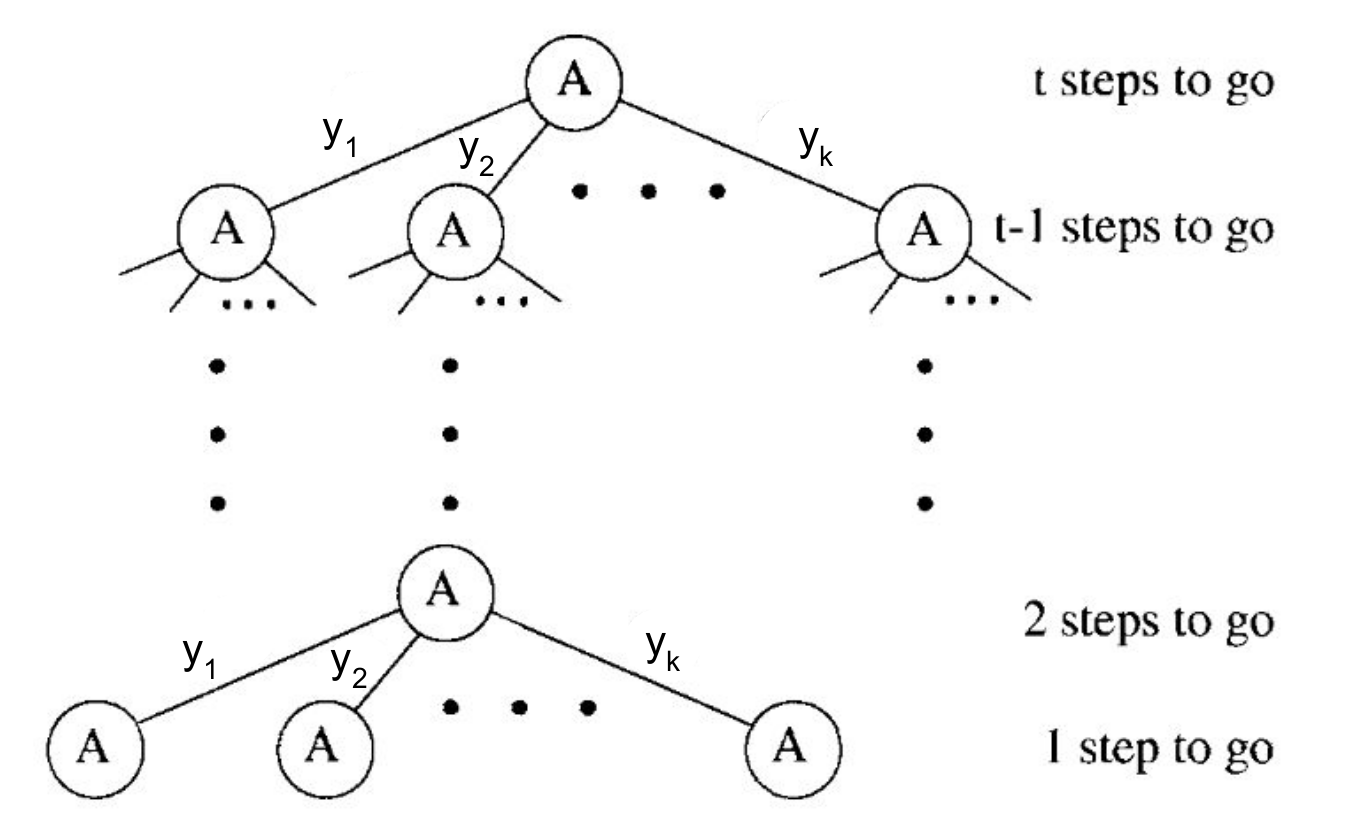
\includegraphics[width=1\linewidth]{figures/policy_tree}
		\caption[A policy tree]{A policy tree of depth t representing t-step nonstationary policy. Source: \cite{KAELBLING199899}}
		\label{fig:policy_tree}
	\end{center}
	\vspace{-40pt}
\end{wrapfigure} 
about the location of the tiger, it might go for opening the door. However, when it has two steps left, it might be wiser to listen and obtain more information about the state of the world.\\
A nonstationary t-step policy can be represented as a \textit{policy tree} shown in \autoref{fig:policy_tree}. The policy tree describes the optimal behaviour for t steps conditioned on the observation. The top node shows the first action to be taken, then depending on the observation, a different branch is followed until the end of the steps. \\\\
The value of a nonstationary t-step tree is given in \autoref{eq:value_func_1}-\autoref{eq:value_of_tree}, where $ s $ is starting state, $ a(p) $ is the first action at the top of the tree, $ s^\prime $ is the next state, and $ y_{i}(p) $ is the (t-1)-step policy that has been choosen after taking the action $ a(p) $ and getting observation $ y_i $. $ \gamma $ is the \textit{discount factor}, such that $ 0\leq \gamma \leq 1 $, used to regulate the contribution of the future rewards to value function \cite{Sutton2018}.
\begin{align} 
V_{p}(s) &=R(s, a(p))+\gamma \cdot(\text { Expected value of the future }) \label{eq:value_func_1}\\
&=R(s, a(p))+\gamma \sum_{s^{\prime} \in \mathcal{S}} \operatorname{Pr}\left(s^{\prime} \mid s, a(p)\right) \sum_{y_{i} \in \mathcal{Y}} \operatorname{Pr}\left(y_{i} \mid s^{\prime}, a(p)\right) V_{y_{i}(p)}\left(s^{\prime}\right) \label{eq:value_func_2}\\
&=R(s, a(p))+\gamma \sum_{s^{\prime} \in \mathcal{S}} T\left(s, a(p), s^{\prime}\right) \sum_{y_{i} \in \mathcal{Y}} \psi\left(s^{\prime}, a(p), y_{i}\right) V_{y_{i}(p)}\left(s^{\prime}\right) 
\label{eq:value_of_tree}
\end{align}
The value of a policy tree $ p $ starting from state $ s $ has two components, as can be seen in \autoref{eq:value_func_1}. The first component is the immediate reward, that is, the reward that the agent will get for taking action $ a(p) $ while at state $ s $. The second component is the expected future reward, discounted by $ \gamma $. This value is computed first by taking the expectation over next possible states $ s^\prime \in \mathcal{S} $, and their values. The value of a state depends on the observation that the agent receives, which will determine the (t-1)-step policy to be executed. Therefore, a second expectation is performed over the observations. \\
As mentioned before, the agent is never certain about the state of the world. Therefore, the relevant value function is that of a policy tree starting from a belief state $ b $, and  calculated as the expected value over the states.
\begin{equation}
V_{p}(b)=\sum_{s \in \mathcal{S}} b(s) V_{p}(s)
\label{eq:value_p_b}
\end{equation}
\autoref{eq:value_p_b} gives the value of a policy tree starting from belief state $ b $. The optimal policy, then, is chosen as the one which has the maximum value. The optimal t-step value starting from belief state $ b $ is executing the best policy tree for that belief state.
\begin{equation}
V_{t}(b)=\max _{p \in \mathcal{P}} V_p(b)
\label{eq:value_t}
\end{equation}
where $ \mathcal{P} $ denotes a finite set of policy trees.
It is noteworthy that the value function of every policy tree $ V_p $ is linear in b. As can be seen from \autoref{eq:value_t}, $ V_t $ is defined as the maximum of all $ V_p $ over b. It is the envelope of these value functions; therefore, it is piecewise-linear and convex.\\
Infinite-horizon discounted model consider the value function over an infinitely long trajectory of the agent. In a POMDP problem, the infinite horizon discounted value function is still convex \cite{White1980}, but it may not always be piecewise-linear. However, it can be approximated by a finite horizon value function for sufficiently many steps \cite{Sawaki1978, Edward2019}.\\
%This model is more realistic and convenient than the finite horizon since usually the number of steps to take is not defined. This models convergence is ensured by a discount factor $ \gamma $ \\
In the problem considered in this thesis, the agent node $ X_{3} $ cannot observe the incoming messages directly, rather a summary of them. This setting presents a POMDP problem. However, since the optimal policy of the agent is assumed to be given, the main focus in the POMDP framework is belief state estimation. \\
In the following, update methods for the belief state are introduced, where belief state refers to the posterior probability distribution over the environment states.

\subsection{Exact Belief State Update}
\label{sec:exact_update}
In a scenario where compact representations of the \textit{transition model}, $ T(s, a, s^{\prime})$,  and \textit{observation model}, $ \psi(s^{\prime}, a, y) $, are available, the belief state update can be obtained as \cite{KAELBLING199899}
\begin{align}
b^{\prime}\left(s^{\prime}\right) &=\operatorname{Pr}\left(s^{\prime} \mid y, a, b\right) \label{eq:bu1}\\
&=\frac{\operatorname{Pr}\left(y \mid s^{\prime}, a, b\right) \operatorname{Pr}\left(s^{\prime} \mid a, b\right)}{\operatorname{Pr}(y \mid a, b)} \label{eq:bu2}\\
&=\frac{\operatorname{Pr}\left(y \mid s^{\prime}, a\right) \sum_{s \in \mathcal{S}} \operatorname{Pr}\left(s^{\prime} \mid a, b, s\right) \operatorname{Pr}(s \mid a, b)}{\operatorname{Pr}(y \mid a, b)}  \label{eq:bu3}\\
&=\frac{\psi\left(s^{\prime}, a, y\right) \sum_{s \in \mathcal{S}} T\left(s,a, s^{\prime}\right) b(s)}{\operatorname{Pr}(y \mid a, b)}.
\label{eq:discrete_belief_update}
\end{align}
The relation between transition model $ T $ and transition intensity matrix $ \textbf{Q} $ can be written as $ T = \exp(t\textbf{Q}) $ from \autoref{eq:ode_sol}. For the derivation above, from \autoref{eq:bu1} to \autoref{eq:bu2}, Bayes' theorem, and from \autoref{eq:bu2} to \autoref{eq:bu3}, law of total probability is applied. It is also noteworthy that the denominator in \autoref{eq:discrete_belief_update} is in the following form, 
\begin{equation}
\operatorname{Pr}(y \mid a, b) = \sum_{\forall s^{\prime} \in \mathcal{S}} \psi(y \mid s^{\prime}, a) \sum_{\forall s \in \mathcal{S}} T(s^{\prime}\mid s,a) b(s)
\label{eq:nasty_denom}
\end{equation}
which is computationally expensive in the case of continuous state space.
\subsection{Exact Belief State Update for CTMP by Filtering}
\label{sec:filtering_CTMC}
Equation \ref{eq:discrete_belief_update} is the discrete-time solution of belief state. However, since in the model described in Section 2.1, the parent nodes are modelled as CTMPs, thus the environment state for the agent is the state of a CTMP, the belief state should be solved in continuous-time. This is achieved by the inference of the posterior probability of CTMP \cite{article}.\\
A \textit{filtering problem} in statistical context refers to the inference of the conditional probability of the true state of the system at a point in time, given the history of observations \cite{Godsill2019}.\\
Let X be a CTMP with transition intensity matrix \textbf{Q}. Assume discrete-time observations denoted by $ y_{1}=y(t_{1}), ..., y_{N}=y(t_{N}) $. The belief state can be written as:
\begin{equation}
b(x_{i};t_{N}) = \operatorname{Pr}(X(t_{N}) = x_{i} \mid y_{1}, ..., y_{N})
\end{equation}
From the master equation given in \autoref{eq:master_equation}, it follows that:
\begin{equation}
\frac{d}{dt} b(x_{j};t)  = \sum_{\forall i} q_{i,j} \cdot b(x_{i};t)
\end{equation}
The time-dependent belief state $ b(t) $ is a row vector with $ \left\lbrace b(x_{i};t)\right\rbrace_{x_{i} \in \rchi}  $.
This posterior probability can be described by a system of ODEs:
%TODO ODE or system of ODEs
\begin{equation}
\frac{db(t)}{dt} = b(t)\textbf{Q}
\end{equation}
where the initial condition $ b(0) $ is a row vector with $ \left\lbrace b(x_{i};t)\right\rbrace_{x_{i} \in \rchi} $ \cite{article}. The solution to this ODE is
\begin{equation}
b(t) = b(0) \exp(t\textbf{Q}).
\label{eq:b_cont}
\end{equation}
The belief state update at discrete times of observation $ y_{t} $ is derived as 
\begin{align}
b(x_{i}; t_{N}) & = \operatorname{Pr}( X(t_{N}) = x_{i},\mid y_{1}, ..., y_{N}) \nonumber\\ & = \frac{\operatorname{Pr}(y_{1}, ..., y_{N}, X(t_{N}) = x_{i})}{\operatorname{Pr}(y_{1}, ..., y_{N})}  \nonumber\\ & = \frac{\operatorname{Pr}(y_{N} \mid y_{1}, ..., y_{N-1}, X(t_{N}) = x_{i})}{\operatorname{Pr}(y_{N} \mid y_{1}, ..., y_{N-1})} \frac{\operatorname{Pr}(y_{1}, ..., y_{N-1}, X(t_{N}) = x_{i})}{\operatorname{Pr}(y_{1}, ..., y_{N-1})}  \nonumber\\ & = Z_{N}^{-1} \ \operatorname{Pr}(y_{N} \mid X(t_{N})=x_{i})\ \operatorname{Pr}( X(t_{N}) = x_{i}\mid y_{1}, ..., y_{N-1})  \nonumber\\ & = Z_{N}^{-1}\ {p(y_{N} \mid x_{i})}\ {b(x_{i}; t_{N}^{-})}
\label{eq:b_jump}
\end{align}
where $ Z_{N} = \sum_{x_{i}\in \rchi} p(y_{N} \mid x_{i})\ b(x_{i}; t_{N}^{-}) $ is the normalization factor \cite{article}.

\subsection{Belief State Update using Particle Filter}
\label{sec:particle_filter}
In a more realistic scenario, the exact update of belief state may not be feasible for several reasons. The computation of exact belief update is expensive for large state spaces, which can be seen from \autoref{eq:nasty_denom}. Moreover, a problem with continuous state spaces requires a belief state represented as probability distributions over an infinite state space rather than a collection of probabilities as given in \cref{sec:exact_update} \cite{Carlo1904}. Such representation cannot be obtained using the exact method. Another reason could be the lack of a compact representation of transition or observation models. Under such circumstances, the belief state is obtained using sample-based approximation methods \cite{Carlo1904}. \\
It should be noted that since the belief state is nothing but the conditional probability of true states given the observations, the problem at hand poses a filtering problem as described in Section \ref{sec:filtering_CTMC}.

\subsubsection{Particle Filtering}
Particle filtering is one of the most commonly used Sequential Monte Carlo (SMC) algorithms. The popularity of this method thrives from the fact that, unlike other approximation methods such as Kalman Filter, it does not assume a linear Gaussian model. This advantage offers great flexibility and finds application in a wide range of areas \cite{Doucet2009}. \\
The key idea in particle filtering is to approximate a target distribution $ p(x) $ by a set of samples, i.e. particles, drawn from that distribution. This is achieved by sequentially updating the particles through two steps. The first step is \textit{importance sampling}. Since the target distribution is not available, the particles are generated from a \textit{proposal distribution} $ q(x) $ and weighted according to the difference between target and proposal distributions. The second step is to resample the particles using these weights with replacement \cite{Godsill2019}. \\
Consider a problem of deriving the expectation $ \hat{f}(x) = \mathbb{E} \left[ f(x)\right] = \int f(x) p(x)dx $, and suppose p(x) is an intractable density function from which the particles cannot be sampled. Instead they are drawn from a proposal distribution q(x), which yields an empirical approximation such that
\begin{align*}
x^{(i)} & \sim q(x) \\
q(x) & \approx \frac{1}{N} \sum_{i=1}^{N} \delta_{x^{(i)}}(x)
\end{align*}
where $ \delta_{x^{(i)}}(x) $ is Dirac delta. The expectation in question can be written as
\begin{align*}
\int f(x) p(x)dx & = \int f(x) \frac{p(x)}{q(x)} q(x)dx\\
\int f(x) \frac{p(x)}{q(x)} \left( \frac{1}{N} \sum_{i=1}^{N} \delta_{x^{(i)}}(x)\right) dx & = \frac{1}{N} \sum_{i=1}^{N}\frac{p(x^{(i)})}{q(x^{(i)})} f(x^{(i)})
\end{align*}
where $ w(x^{(i)}) = \frac{p(x^{(i)})}{q(x^{(i)})} $ is defined as \textit{importance weight} of a particle. Then the particles are resampled using the importance weights with replacement, which concludes one iteration of sequential updating \cite{Godsill2019}.\\
%TODO something like, the proposal distribution is marginalized distribution of CTBN, relate the following to the example.

\subsubsection{Marginalized Continuous-Time Markov Processes}
\label{sec:marg_ctbn}
In this work, the particles to represent the belief state are drawn from a marginalized CTBN. Consider a CTBN, S, with local variables $ X_n $, $ n\in \left\lbrace 1,...,N \right\rbrace $, and a set of conditional intensity matrices \textbf{\textit{Q}}. In the following, it is assumed that every non-diagonal entry in $ \textbf{Q}_{n\mid u} $ is Gamma distributed with shape and rate parameters, $ \alpha^n_{i,j\mid u} $ and $ \beta^n_{i,j\mid u} $.\\
The marginal process description of S considering a single trajectory in the interval $ [0,t) $ can be written as
\begin{align}
\operatorname{Pr}(X_n(t &+ h) = x_j \mid X_n(t)=x_i, U_n(t)=u, S^{[0, t)})\\
&= \int \operatorname{Pr}(X_n(t + h) = x_j \mid X_n(t)=x_i, U_n(t)=u, Q_{n\mid u}, S^{[0, t)})p(Q_{n\mid u})dQ_{n\mid u}\\
&= \delta_{i,j} + \mathbb{E}[q^n_{i,j\mid u} \mid S^{[0, t]} = s^{[0, t]}]\ h + o(h).
\label{eq:marginal_CTBN}
\end{align}
By integrating out the intensity matrix $ Q_{n\mid u} $, the parameter is replaced by its expected value given the history of the process. It should be noted that by doing so, the process becomes parameter-free, and thus self-exciting \cite{Studer2016}. \\
The derivation of the conditional expectation for a marginal CTBN follows from the Bayes' rule:
\begin{equation}
p\left(\textbf{Q} \mid S^{[0,t]}\right)=\frac{p\left(S^{[0,t]} \mid \textbf{Q}\right) p(\textbf{Q})}{p\left(S^{[0,t]}\right)}
\label{eq:Q_bayes}
\end{equation}
\autoref{eq:Q_bayes}, written for single trajectory $ S^{[0,t]} $, can be extended for multiple trajectories. Consider K trajectories drawn from S, denoted by $ \xi_t = \left\lbrace S^{[0,t], 1}, S^{[0,t], 2}, ..., S^{[0,t], K} \right\rbrace  $. Since the trajectories are conditionally independent, given \textbf{Q}, using \autoref{eq:lh_CTBN} the likelihood of set $ \xi_t $ is written as,
\begin{align}
\operatorname{Pr}( \xi_t  \mid \textbf{\textit{Q}} ) = \prod_{n=1}^{N} \prod_{u \in \mathcal{U}_{n}} \prod_{x_i \in \mathcal{X}_{n}} \prod_{x_j \in \mathcal{X}_{n} \backslash x_i}
\exp \left( q_{i,j\mid u}^{n} T_{n}[x_i\mid u]\right) (q_{i,j\mid u}^{n})^{M_{n}[x_i, x_j\mid u]}
\label{eq:lh_dataset_CTBN}
\end{align}
where the joint sufficient statistics of $ X_n $ over all K trajectories are denoted by  $ T_{n}[x_i\mid u] = \sum_{k=1}^{K} T_{n}^k[x_i\mid u] $ and $ M_{n}[x_i, x_j\mid u] =\sum_{k=1}^{K} M_{n}^k[x_i, x_j\mid u]$.\\
Given independent Gamma-priors on transition intensities, the expectation in \autoref{eq:marginal_CTBN} can be evaluated as follows:
\begin{equation}
\mathbb{E}\left[q_{i,j\mid u}^{n} \mid \xi_{t}\right]=\frac{\alpha^n_{i,j\mid u}+M_{n}[x_i, x_j\mid u]}{\beta^n_{i,j\mid u}+T_{n}[x_i \mid u]}
\label{eq:estimated_Q}
\end{equation}
The algorithm for belief state update through marginal particle filtering is given in the following chapter. 
%TODO: when is this parameter updated? Explain. Write about the dependency problem; how is this okay?

\section{Sampling Algorithms}
\label{sec:sampling_alg}
\subsection{Gillespie Algorithm for Generative CTBN}
Gillespie algorithm is a computer-oriented Monte Carlo simulation procedure that is originally proposed to simulate the reactions of molecules in any spatially homogeneous chemical system. Such systems are regarded as Markov processes and represented via their master equations, which cannot be directly used to obtain realizations of the process. Gillespie algorithm is an efficient tool to overcome this problem \cite{Gillespie1976}.\\
This algorithm can also be applied to sample \textit{events} from a CTBN given the transition intensity matrices, where an event refers to a transition occurring at a specific point in time. This procedure is introduced as \textit{Generative CTBN} in \cite{Nodelman1995}.


\begin{algorithm}[H]
	\SetKwInOut{KwIn}{Input}
	\SetKwInOut{KwOut}{Output}
	\SetKwInOut{Init}{Initialize}
	
	\KwIn{Structure of the network with N local variables $ X_{1}, X_{2}, ..., X_{n} $ with state-space $ \rchi_n = \left\lbrace x_{1}, ..., x_{m} \right\rbrace $   \\Transition intensity matrices $ \textbf{Q}_{n} $ with entries $ q^n_{i,j}$\\$ T_{max} $ to terminate simulation}
	\KwOut{Sample trajectory of the network}
	\Init{Initialize node values $ X_{n}(0) = x_{i} \in \rchi_n$}
	
	\begin{algorithmic}[1]
		\WHILE{$ t < T_{max} $}
		\STATE{$ \tau \sim \exp(\sum_{\forall n} \sum_{\forall i \neq j} \ q^{n}_{i,j}) $}
		\STATE{\text{transitioning node is randomly drawn with probability}  $ P(X_{n}) = \frac{q^{n}_{i}}{\sum_{\forall n} q^{n}_{i}}$}
		\STATE{\text{next state is randomly drawn with probability} $ P(x_{j}) = \frac{q^{n}_{i,j}}{q^{n}_{i}} $}
		\STATE{$ t \leftarrow t + \tau $}
		\ENDWHILE
	\end{algorithmic}
	\caption{Generative CTBN}
	\label{alg:generative_ctbn}
\end{algorithm}

\subsection{Thinning Algorithm}
Thinning algorithm is a method introduced to simulate nonhomogenous Poisson processes \cite{Lewis1979}. Later, it is adapted to sample from Hawkes processes, a self-exciting process with time-dependent intensity function \cite{Ogaata1981, Rizoiu2017}. This algorithm is used here to simulate the inhomogeneous Markov process.

\begin{algorithm}[H]
	\SetKwInOut{KwIn}{Input}
	\SetKwInOut{KwOut}{Output}
	\SetKwInOut{Init}{Initialize}
	
	\KwIn{$\lambda(t)$ the intensity function of the inhomogenous process  \\ $ N $ number of events to terminate simulation}
	\KwOut{Sample trajectory of the process}
	\Init{Time $ t = 0 $}
	
	\begin{algorithmic}[1]
		\WHILE{$ i < N $}
		\STATE{\text{the upper bound for intensity,} $ \lambda^{*}$}
		\STATE{\text{transition time $ \tau $ drawn by }  $ u \sim U(0, 1)$ \textit{ and } $ \tau = \frac{-ln(u)}{\lambda^{*}} $}
		\STATE{$ t \leftarrow t + \tau $}
		\STATE{\text{draw } $s \sim U(0, 1)$}
		\IF{ $ s \leq \frac{\lambda(t)}{\lambda^{*}}$}
		\STATE{\text{sample accepted and } $ t_i = t$, $ i=i+1 $}
		\ENDIF
		\ENDWHILE
	\end{algorithmic}
	\caption{Thinning Algorithm}
\end{algorithm}